While ordinary Internet users request mainly optimized  web sites to make the
most of each user connection, it is natural that the traffic generated by
several requests of web sites simultaneously generates some kind of significant
load to the network. Or so it is what one should naturally think.

Unfortunately with the results obtained with this Page Benchmark it is 
clear it is not so. By analyzing Figure \ref{fig:loadmeans}, the
networks that already were categorized as \emph{with problems}, follow that
trend and even with all the available bandwidth, take longer to complete the
request. As example, the network \emph{marcia\_w} without other sources of
load took a little over 9 seconds to complete the site request \footnote
{Again, the website is \url{http:// www.usm.cl}}. This results is way above
expectations since under normal conditions, the normal average is between 1-7
seconds with a tendency to be close to 2 seconds). An important study case of
study is the network \emph{mbahamon\_w} which was one of the lowest overall
in cases without overloading the network. While on a later date after these
tests, it was necessary to change the router used as access point, which
generated a lot of noise and interference for testing between tests seeing
themselves in a bad state at that time.

\begin{figure}[ht]
\centering
	%\rule{5.5cm}{7.1cm}
    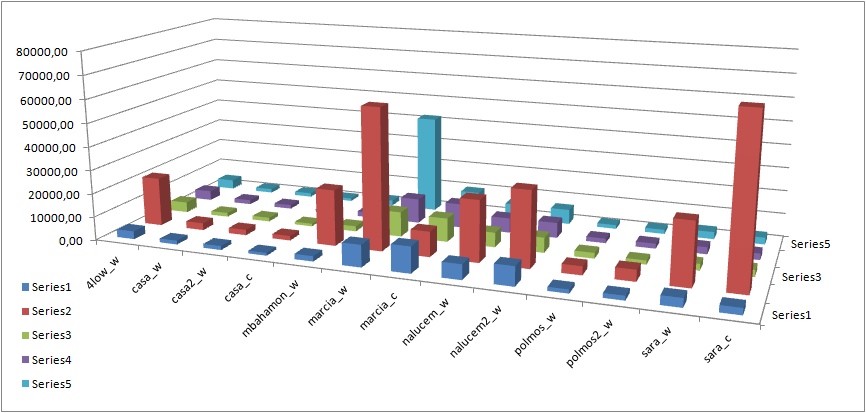
\includegraphics[width=0.9\textwidth]{img/measures_page}
\caption[Page Benchmark: Total Load Means]{ Total Load means (in ms) based on \ref{app:pbmeasures}, Table \ref{table:loadmeans}}
\label{fig:loadmeans}
\end{figure}%

Before realizing that the router was the flaw in the network
\emph{mbahamon\_w}, under conditions of stress, this network was one of the
most affected networks delaying average time 23 seconds. The networks that are
in worst situations are those mentioned \emph{marcia\_w} and
\emph{sara\_c}. Due to the presence of large buffers which store packets of
uncontrolled manner and for longer periods, when the network's load decreases,
this resource  still under utilization. This is reflected in the observations
from from 3 onwards.

\begin{table}[ht]
\begin{center}
\begin{tabular}{|c||c|c|c||}
 \hline
Name 			& min		& max		& ratio  	\\ \hline \hline
4low\_w 		& 3415,1	& 20932,3	& 612,93374 \\ \hline 
casa\_w 		& 1654,8	& 3053,6	& 184,52985 \\ \hline 
casa2\_w		& 1646,6	& 2354,4	& 142,98555	\\ \hline 
casa\_c			& 1165,3	& 1944,1	& 166,83258	\\ \hline 
mbahamon\_w		& 2182,6	& 23868,5	& 1093,58105\\ \hline 
marcia\_w		& 9401,6	& 60119,0	& 639,45499	\\ \hline 
marcia\_c		& 10028,3	& 11140,0	& 111,08563	\\ \hline 
nalucem\_w 		& 6280,8	& 26048,6	& 414,73379	\\ \hline 
nalucem2\_w 	& 6349,4	& 32151,5	& 506,37068	\\ \hline 
polmos\_w 		& 1623,4	& 3701,4	& 228,00296	\\ \hline 
polmos2\_w 		& 1738,5	& 4861,8	& 279,65487	\\ \hline 
sara\_w 		& 2808,6	& 26561,5	& 945,72029	\\ \hline 
sara\_c 		& 2757,6	& 70423,3	& 2553,78953\\ \hline 
\end{tabular}
\caption[Page Benchmark: Minimum, Maximum and variation ratio.]{Minimum, Maximum and variation ratio.}
\label{table:varatio}
\end{center}
\end{table}

In Table \ref{table:varatio}, can be seen the comparison between the minimum
and maximum average load value across over all iterations on the same network
and the ratio between these values. While the ratio can not be compared
directly between two different networks, but can compare how many times the
maximum value was respect to its original value \footnote{a network may have a
low ratio with times that have a low variance and high average time}. Here,
the network \emph{marcia\_c}, and in the Table \ref{table:loadmeans},
accomplish times that were close to 11 seconds for all five iterations. With
this values, the ratio is low (11\%) but the real values are relatively high
for normal conditions (around 11 seconds).

Again, the networks \emph{marcia\_w}, both cases for \emph{sara}, stand
here because the high level of variation around 6 to 20 times the lowest
average time; highlighting \emph{mbahamon\_w} and \emph{sara\_c}. Contrary
to what was expected, in the case of the wired iteration over sara,
\emph{sara\_c}, the maximum variation was significantly higher in this
iterations than for those observed using wireless technology.

\begin{table}[!ht]
\begin{center}
\begin{tabular}{|c||c|c|c|c|c||}
 \hline
 & \multicolumn{5}{|c|}{ Ratio (\%)} \\ \hline
Name 		& 1			& 2			 & 3	        & 4				& 5 			\\ \hline \hline
4low\_w		& 155,55556	& 707,62342	 & 196,64754	& 232,87492		& 3302,32392	\\ \hline
casa\_w		& 108,35366	& 299,26429	 & 116,08775	& 356,49786		& 118,85296 	\\ \hline
casa2\_w	& 113,99878	& 281,65249	 & 127,18041	& 103,10219		& 117,71533 	\\ \hline
casa\_c		& 112,57589	& 304,73684	 & 103,63636	& 103,57766		& 104,58478 	\\ \hline
mbahamon\_w	& 163,95912	& 183,86356	 & 153,77847	& 139,55813		& 319,52128 	\\ \hline
marcia\_w	& 309,24808	& 6298,01469 & 267,57064	& 198,10685		& 205,48759 	\\ \hline
marcia\_c	& 310,36182	& 187,34044	 & 146,11202	& 205,08497		& 138,25129 	\\ \hline
nalucem\_w	& 261,95410	& 254,73473	 & 109,85803	& 106,96041		& 105,23376 	\\ \hline
nalucem2\_w	& 980,66263	& 315,95548	 & 254,12946	& 284,86443		& 110,70346 	\\ \hline
polmos\_w	& 106,36537	& 263,10680	 & 3902,47219	& 8443,23607	& 4150,06459 	\\ \hline
polmos2\_w	& 159,75460	& 1991,19249 & 8206,53009	& 417,45121		& 8226,29199 	\\ \hline
sara\_w		& 402,38095	& 240,75420	 & 394,93299	& 976,89312		& 395,52042 	\\ \hline
sara\_c		& 111,04952	& 281,07638	 & 109,03226	& 107,01366		& 109,54898 	\\ \hline
\end{tabular}
\caption[Page Benchmark: Ratio over own iteration]{Ratio over own iteration.}
\label{table:variationratio}
\end{center}
\end{table}

Also, for some cases adding another source was not decisive to obtain times
quite high. As can be seen in \ref{table:variationratio}, for
\emph{polmos\_w}, which in its latest iteration had a maximum of 127.343 ms
\footnote{The detailed values are available with CD} and a minimum of 1548ms.
Grounds for these outlayers measurements may be due to many factors ranging
from the conection setup to server problems.
